\subsection{Signal and Systems}
\subsubsection{Classification of Signals}   
\begin{enumerate}
    \item Unit Step Function
    \begin{equation}
    u(t) = 
        \begin{cases}
             & \text{1; t $\geq$ 0}\\
             & \text{0: t $\leq$ 0}\\
        \end{cases}
    \end{equation}
    \begin{figure}[h]
        \centering
        \includegraphics[width=0.6\textwidth]{image/image.png}
        \label{fig:enter-label}
    \end{figure}
    \item Sign (or Signum) function
    \begin{equation}
    sgn(t) = 
        \begin{cases}
            & +1; t \geq 0 \\
            & -1; t < 0
        \end{cases}
    \end{equation}
    \begin{figure}[h]
        \centering
        \includegraphics[width=0.5\textwidth, height=4cm]{image/Signum_function.svg.png}
        \label{fig:enter-label}
    \end{figure}
    \newpage    
    \item Rectangle Function
    \begin{equation}
    rect(\frac{t}{T}) = 
        \begin{cases}
            & 1; \frac{T}{2}\leq t < \frac{T}{2} \\
            & 0; \text{elsewhere}
        \end{cases}
    \end{equation}
    \begin{figure}[h]
        \centering
        \includegraphics[width=0.6\textwidth]{image/1920px-Rectangular_function.svg.png}
        \label{fig:enter-label}
    \end{figure}
    \item Triangle function
    \begin{equation}
    tri(\frac{t}{T}) = 
        \begin{cases}
            & 1-\frac{|t|}{T};  |t|\leq T \\
            & 0;                |t|\geq T
        \end{cases}
    \end{equation}
    \begin{figure}[h]
        \centering
        \includegraphics[width=0.6\textwidth]{image/Triangular_function.svg.png}
        \label{fig:enter-label}
    \end{figure}
    \newpage
    \item Sinc Function
    \begin{equation}
    sinc(\frac{t}{T}) = 
        \begin{cases}
            & \frac{sin(\frac{\pi t}{T})}{\frac{\pi t}{T}} ;  t \neq 0\\
            & 1 ; t \neq 0
        \end{cases}
    \end{equation}
    \begin{figure}[h]
        \centering
        \includegraphics[width=0.6\textwidth]{image/sinc.png}
        \label{fig:enter-label}
    \end{figure}
    \\
    Take note that when calculate $sinc(x) = 0$ make sure, the $\frac{t}{T}$ in $sin(\frac{\pi t}{T})$ is integer so that $sin$ is zero, $sinc(x)$ will be zero.
    \item Two-Sided decaying exponential function
    \begin{equation}
        e^{-\alpha |t|} ; a > 0
    \end{equation}
    \begin{figure}[h]
        \centering
        \includegraphics[width=0.6\textwidth]{image/exponential.jpg}
        \label{fig:enter-label}
    \end{figure}
    \item Right-Sided decaying exponential function
    \begin{equation}
        e^{-\alpha t}u(t) = 
        \begin{cases}
            & e^{-\alpha t} ; t \geq 0 \\
            & 0 ; t < 0 ;
        \end{cases}
    \end{equation}
    \item Sinusoidal Signals
    \begin{equation}
        x(t) = \mu cos(\omega_0t+\phi) = \frac{\mu}{2}[e^{j\omega_0t+\phi}+e^{-j(\omega_0t+\phi)}]
    \end{equation}
    \begin{equation}
        x(t) = \mu sin(\omega_0t+\phi) = \frac{\mu}{j2}[e^{j\omega_0t+\phi}-e^{-j(\omega_0t+\phi)}]
    \end{equation}
    \begin{equation}
        x(t) = \mu e^{j(\omega_0t+\phi)} = \mu[cos(\omega_0t+\phi) + jsin(\omega_0t+\phi)]
    \end{equation}
    Where \\
    $\mu > 0$ : Magnitude \\
    $\omega_0$ : angular frequency ($rad/s$)\\
    $\phi$ : phases (radian) \\
    $\omega_0t + \phi$ : instantaneous phase \\
    Take note that it is commonly replace $\omega_0$ with $2\pi f_0$ where $f_0$ is the cyclic frequency. \\
    The fundamental period $T_0$ is given by \[T_0 = \frac{2\pi}{\omega_0} = \frac{1}{f_0}\]
\end{enumerate}

\subsubsection{Time-domain Operations and Dirac Impulse}
\begin{enumerate}
    \item Time-scaling, time-shifting \\
    Lets say we have a signal $x(t)$, for $y(t) = \alpha x(\gamma t - \beta)$, where $\alpha$ is time-scaling factor and $\beta$ is time-shifting factor. To draw the signal $y(t)$, all y-coordinates should times $\alpha$ and all x-coordinates should plus $\beta$. The $\gamma$ is a stretching factor that all x-coordinates will be stretched by times $\frac{1}{\gamma}$.  
    \item Sum of two signals \\
    Given two signals to sum up. You should add all corresponding y-coordinates of each signal's 
    x-coordinates to form your new y-coordinates. 
    \newpage
    For example:
    \begin{figure}[h]
        \centering
        \includegraphics[width=1\textwidth]{image/triangle_add_example.jpg}
        \label{fig:enter-label}
    \end{figure}
    \item Multiplication of two signals
    \begin{figure}[h]
        \centering
        \includegraphics[width=0.9\textwidth]{image/mutiplication.jpg}
        \label{fig:enter-label}
    \end{figure}
    \item Convolution of two signals
    \begin{equation}
        x(t)*y(t) = \int^{\infty}_{\infty}x(\alpha)y(t-\alpha)d\alpha
    \end{equation}
    \newpage
    \item Dirac-$\delta$ Impulse
    \begin{itemize}
        \item The Dirac-$\delta$ function is known as \textit{unit impulse}, is defined by
        \begin{equation}
            \delta(t) = 
            \begin{cases}
                & \infty ; t = 0\\
                & 0      ; t \neq 0
            \end{cases}
        \end{equation}
    and 
    \begin{equation}
        \int^{\varepsilon}_{-\varepsilon}\delta(t)\, dt = 1 \;\; \forall\varepsilon > 0
    \end{equation}
    \item Property of $\delta(t)$ function
        \begin{enumerate}
            \item Symmetry : $\delta(t) = \delta(-t)$
            \item Sampling : $x(t)\delta(t-\lambda) = x(\lambda)\delta(t-\lambda)$
            \item Sifting : $\int^{\infty}_{-\infty}x(t)\delta(t-\lambda)dt = x(\lambda)\int^{\infty}_{-\infty}\delta(t-\lambda)dt = x(\lambda)$
            \item Replication : $x(t)*\delta(t-\lambda) = x(t-\lambda)$
        \end{enumerate}
    \end{itemize}
    \item Dirac-$\delta$ Comb Function a.k.a Sampling function
    \begin{equation}
        \sum^{\infty}_{n=-\infty}\delta(t-nT) = \dots + \delta(t+2T)+\delta(t+T)+\delta(t)+\delta(t-T)+\dots
    \end{equation}
    \begin{itemize}
        \item Replication
            \[x_p(t) = x(t)*\sum_{n}\delta(t-nT_p) = \sum_n x(t- nT_p)\]
        \item Sampling
            \[x_s(t) = x(t)\times\sum_n\delta(t-nT_s)=\sum_n x(nT_s)\delta(t - nT_s)\]
    \end{itemize}
\end{enumerate}

\subsubsection{Energy Signal and Power Signal}
\begin{enumerate}
    \item Energy Signals
    \begin{itemize}
        \item The total energy of a signal is defined as 
        \[E = \int^{\infty}_{-\infty}|x(t)|^2dt\]
        \item $x(t)$ is said to be an energy signal if $0<E<\infty$.
    \end{itemize}
    \item Power Signal
    \begin{itemize}
        \item The Average Power of a signal is defined as
        \[P = \lim_{\tau\rightarrow\infty}\frac{1}{2\tau}\int^{\tau}_{-\tau}|x(t)|^2dt\]
        \item $x(t)$ is said to be a power signal if $0<P<\infty$.
    \end{itemize}
\end{enumerate}

\subsubsection{Discrete-Frequency Spectrum}
\begin{enumerate}
    \item Spectrum of Sinusoid \\
    A spectrum of complex sinusoidal signal can be represented by 
    \[ \tilde{x(t)} = \mu e^{j(2\pi f_0t + \phi)} = \mu e^{j\phi}\times e^{j2\pi f_0 t}\]
    From this, you can draw your Magnitude spectrum and Phase spectrum. \\
    For example, 
    \begin{figure}[h]
        \centering
        \includegraphics[width=0.9\textwidth]{image/magnitude_example.jpg}
        \label{fig:enter-label}
    \end{figure}
    \item Fourier Series \\
    For any bounded periodic signal, $x_p(t)$, with period $T_p$ can be represented by a sum of harmonically related complex sinusoidal.
    \begin{equation}
        x_p(t) = \sum^{\infty}_{k=-\infty}c_k e^{j2\pi k \frac{t}{T_p}} = \sum^{\infty}_{k=-\infty}c_k e^{j2\pi kf_p t}
    \end{equation}
    where $f_p = \frac{1}{T_p}$ is the fundamental frequency of $x_p(t)$, and $kf_p$ is the $k^{th}$ harmonic of $f_p$. \\
    $c_k$ are called \textit{Fourier series coefficients} of $x_p(t)$. \\
    The function to determine $c_k$ are given by
    \begin{equation}
        c_k = \frac{1}{T_p}\int^{t_0+T_p}_{t_0}x_p(t)e^{-j2\pi k \frac{t}{T_p}}dt, \; k=0,\pm1, \pm2, \dots
    \end{equation}
    \item Trigonometric Fourier Series
    \begin{equation}
        x_p(t) = a_0 + 2\sum^{\infty}_{k=1}[a_k cos(2\pi k \frac{t}{T_p})+b_ksin(2\pi k \frac{t}{T_p})]
    \end{equation}
    where $a_k$ and $b_k$ are given by
    \[a_k = \frac{1}{T_p}\int^{t_0+T_p}_{t_0}x_p(t)cos(2\pi k \frac{t}{T_p}); \; k > 0\]
    \[b_k = \frac{1}{T_p}\int^{t_0+T_p}_{t_0}x_p(t)sin(2\pi k \frac{t}{T_p}); \; k > 0\]
\end{enumerate}
\subsubsection{Continuous-Frequency Spectrum} 
The Fourier Series expansion for a aperiodic signal does not exist. In this case, we make use of \textit{Fourier Transform} to derive the spectrum of a aperiodic signal in the continuous-frequency domain, $f$ .
\begin{enumerate}
    \item Fourier Transform \\
    \begin{equation}
        X(f) = \int^{\infty}_{-\infty}x(t)e^{-j2\pi ft}dt
    \end{equation}
    The inverse of Fourier transform is given by
    \begin{equation}
        x(t) = \int^{\infty}_{-\infty}X(f)e^{j2\pi ft}df
    \end{equation}
    \item Conditions for Fourier transformation (\textbf{Dirichlet Condition})
    \begin{itemize}
        \item $x(t)$ only has finite number of maxima and minima in any finite time interval.
        \item $x(t)$ only has finite number of discontinuities in any finite time interval.
        \item $x(t)$ is absolute integrable. For e.g. $\int^{\infty}_{-\infty}|x(t)| dt < \infty$
    \end{itemize}
    Note that point 3 is satisfied by most energy signals and violated by all power signals.
    \item Property of Fourier Transform
    \begin{enumerate}
        \item Linearity
        \begin{equation}
            \alpha x_1(t)+\beta x_2(t) \Longleftrightarrow \alpha X_1(f) + \beta X_2(f)
        \end{equation}
        \item Time Scaling
        \begin{equation}
            x(\beta t) \Longleftrightarrow \frac{1}{|\beta|}X(\frac{f}{\beta})
        \end{equation}
        \item Duality
        \begin{equation}
            X(t) \Longleftrightarrow x(-f)
        \end{equation}
        \item Time Shifting
        \begin{equation}
            x(t-t_0) \Longleftrightarrow X(f)e^{-j2\pi ft_0}
        \end{equation}
        \item Frequency Shifting
        \begin{equation}
            X(f-f_0) \Longleftrightarrow x(t)e^{j2\pi f_0t}
        \end{equation}
        \item Differentiation in the Time Domain
        \begin{equation}
            \frac{d}{dx}x(t) \Longleftrightarrow j2\pi f \cdot X(f)
        \end{equation}
        \item Integration in the Time Domain
        \begin{equation}
            \int^t_{-\infty}x(\tau)d\tau \Longleftrightarrow \frac{1}{j2\pi f}X(f)+\frac{1}{2}X(0)\delta(f) 
        \end{equation}
        \item Convolution in Time Domain
        \begin{equation}
            \underbrace{\int^{\infty}_{-\infty}x_1(\alpha)x_2(t-\alpha)d\alpha}_\text{$x_1(t)*x_2(t)$}\Longleftrightarrow X_1(f)X_2(f)
        \end{equation}
        \item Multiplication in Time Domain
        \begin{equation}
            x_1(t)x_2(t)\Longleftrightarrow \underbrace{\int^{\infty}_{-\infty}X_1(\alpha)X_2(f-\alpha)d\alpha}_\text{$X_1(f)*X_2(f)$}
        \end{equation}
    \end{enumerate}
    \newpage
    \item Fourier Transform of Basic Functions
    \begin{table}[h]
        \setlength{\arrayrulewidth}{0.3mm}
        \renewcommand{\arraystretch}{1.93}
        \centering
        \begin{tabular}{|c|c|c|}
        \hline
        &   $x(t)$     & $X(f)$ \\
        \hline
        Constant & $K$ & $K\delta(t)$ \\
        \hline
        Unit Impulse & $\delta(t)$ & $1$ \\
        \hline
        Unit Step & $u(t)$ & $\displaystyle \frac{1}{2}[\delta(f) + \frac{1}{j\pi f}]$ \\
        \hline
        Sign (Signum) & $sgn(t)$ & $\displaystyle \frac{1}{j\pi f}$ \\
        \hline
        Rectangle & $rect(\frac{t}{T})$ & $Tsinc(fT)$ \\
        \hline
        Triangle & $tri(\frac{t}{T})$ & $Tsinc^2(fT)$ \\
        \hline
        Sine Cardinal & $sinc(\frac{t}{T})$ & $Trect(fT)$ \\
        \hline
        Complex Exponential & $e^{j2\pi f_0 t}$ & $\delta(f-f_0)$ \\
        \hline
        Cosine & $cos(2\pi f_0t)$ & $\displaystyle \frac{1}{2}[\delta(f-f_0)+\delta(f+f_0)]$\\
        \hline
        Sine & $sin(2\pi f_0t)$ & $\displaystyle \frac{-j}{2}[\delta(f-f_0)-\delta(f+f_0)]$\\
        \hline
        Gaussian & $\displaystyle e^{-\frac{t^2}{\alpha^2}}$ & $\displaystyle \alpha \pi^{0.5}e^{\alpha^2\pi^2f^2}$ \\
        \hline
        Comb & $\displaystyle \sum^{\infty}_{m=-\infty}\delta(t-mT)$ & $\displaystyle \frac{1}{T}\sum^{\infty}_{k=-\infty}\delta(f-\frac{k}{T})$\\
        \hline
        \end{tabular}
        \caption{Fourier Transform Table}
        \label{tab:my_label}
    \end{table}
\end{enumerate}
\subsubsection{Spectral Density and Bandwidth}
\begin{enumerate}
    \item  Energy Spectrum Density (ESD) \\
    Energy spectral density describes how the total energy of a signal is distributed in the frequency domain. The Rayleigh’s energy theorem provides us with an alternate method for computing the total energy of a signal in the frequency-domain, namely
    \begin{equation}
        E = \int^{\infty}_{-\infty}|x(t)|^2dt = \int^{\infty}_{-\infty}|X(f)|^2df \; \text{$\cdots$\textbf{Rayleigh Energy Theorem}}
    \end{equation}
    The Energy Spectrum Density is 
    \begin{equation}
        E_x(f) = |X(f)|^2
    \end{equation}
    \item Property of \textbf{ESD} 
        \begin{enumerate}
            \item $E_x(f)$ is a real function of f
            \item $E_x(f) \geq 0 \;\; \forall f$
            \item $E_x(f)$ is an even function of $f$ if $x(t)$ is real
        \end{enumerate}
    \item Power Spectrum Density (PSD) \\
    For continuous-time signals that have infinite total energy, for example power signals, it makes more sense to define a power spectral density, which describes how the average power of a signal is distributed in the frequency domain.\\
    The \textbf{Parseval power theorem} is given by
    \begin{equation}
        P = \underbrace{\lim_{W\rightarrow\infty}\frac{1}{2W}\int^W_{-W}|x(t)|^2dt}_\text{Average Power} = \int^{\infty}_{-\infty}\lim_{W\rightarrow\infty}\frac{1}{2W}|X_W(f)|^2df
    \end{equation}
    The Power Spectrum Density
    \begin{equation}
        P_x(f) = \lim_{W\rightarrow\infty}\frac{1}{2W}|X_W(f)|^2df
    \end{equation}
    \item Property of \textbf{PSD}
        \begin{enumerate}
            \item $P_x(f)$ is a real function of f
            \item $P_x(f) \geq 0 \;\; \forall f$
            \item $P_x(f)$ is an even function of $f$ if $x(t)$ is real
        \end{enumerate}
    \item PSD for Periodic Signal\\
    Given a $x_p(t)$ is periodic, the spectrum of $x_p(t)$ is given by
    \[X_p(f) = \sum^{\infty}_{k=-\infty}c_k\delta(f-kf_p)\]
    The \textbf{Power Spectrum Density of $x_p(t)$} is
    \[P_x(f) = \sum^{\infty}_{k=-\infty}|c_k|^2\delta(f-kf_p) \]
    The \textbf{Average Power of $x_p(t)$} is 
    \[P = \int^{\infty}_{-\infty}P_x(f)\;df = \sum^{\infty}_{k=-\infty}|c_k|^2\]
    \item Bandwidth
    \begin{enumerate}
        \item Lowpass Signal\\
        A signal $x(t)$ is said to be a bandlimited lowpass signal if its magnitude spectrum is concentrated around $0 Hz$ , and at the same time satisfies
        \[|X(f)| = 0 ; \; |f| > B\]
        where B is defined as the bandwidth of the signal
        \item Bandpass Signal \\
        A signal $x(t)$ is said to be a bandlimited bandpass signal if its magnitude spectrum is concentrated around a non-zero center frequency, $f_c$ , and at the same time satisfies
        \[|X(f)| = 0 ; \; ||f| -f_c|> \frac{B}{2}\]
        \item \textbf{3dB} Bandwidth \\
        The 3dB bandwidth of $x(t)$ is defined as the frequency where 
        \[X(f) = \frac{|X(0)|}{\sqrt{2}}\; or \; |X(f)| = \sqrt{X(f)X^*(f)} \; or \; \frac{E_x(f_B)}{E_x(0)} = \frac{|X(f_B)|^2}{|X(0)|^2} = \frac{1}{2}\]
        first occurs when $f$ is increased from 0 Hz
        \item \textbf{$1^{st}-null$} Bandwidth \\
        The $1^{st}$-null bandwidth of a lowpass signal $x(t)$ is defined as the frequency at which 
        \[X(f) = 0\]
        first occurs when f increased from 0 Hz
    \end{enumerate}
    \item \textbf{M\%} Energy Containment Bandwidth \\
    The M\% energy containment bandwidth, $B$, of a real energy signal is the smallest bandwidth that contains at least M\% of the total energy 
    \[\int^{f_B}_{-f_B}E_x(f)\;df = \frac{M}{100}\times E\]
    \item \textbf{M\%} Power Containment Bandwidth \\
    The M\% power containment bandwidth, $B$, of a real energy signal is the smallest bandwidth that contains at least M\% of the average signal power. The M\% power containment bandwidth, $B$, is given by $B = Kf_p$, where K is the smallest positive integer that satisfies 
    \[\sum^{K}_{k=-K}|c_k|^2\geq\frac{M}{100}\times P\]
\end{enumerate}
\newpage
\subsubsection{Classification and s-Domain Analysis}
\begin{enumerate}
    \item Laplace Transformation
        \begin{table}[h]
            \setlength{\arrayrulewidth}{0.3mm}
            \renewcommand{\arraystretch}{1.93}
            \centering
            \begin{tabular}{|c|c|c|}
            \hline
               & $f(t)$ & $\tilde{F}(s)$ \\
            \hline
            Unit Impulse & $\delta(t)$ & $1$ \\
            \hline
            Unit Step & $u(t)$ & $\displaystyle\frac{1}{s}$ \\
            \hline
            Ramp & $tu(t)$ & $\displaystyle \frac{1}{s^2}$ \\
            \hline
            $n^{th}$ order Ramp & $t^nu(t)$ & $\displaystyle \frac{n!}{s^{n+1}}$ \\
            \hline
            Damped Ramp & $\displaystyle te^{-\alpha t}u(t)$ & $\displaystyle \frac{1}{(s+\alpha)^2}$ \\
            \hline
            Exponential & $\displaystyle e^{-\alpha t}u(t)$ & $\displaystyle\frac{1}{s+\alpha}$ \\
            \hline
            Cosine & $cos(\omega_0t)u(t)$ & $\displaystyle \frac{s}{(s^2+\omega_0^2)}$\\
            \hline
            Sine & $sin(\omega_0t)u(t)$ & $\displaystyle \frac{\omega_0}{(s^2+\omega_0^2)}$\\
            \hline
            Damped Cosine & $\displaystyle e^{-\alpha t}cos(\omega_0t)u(t)$ & $\displaystyle \frac{s+\alpha}{(s+\alpha)^2+\omega_0^2}$ \\
            \hline
            Damped Sine & $\displaystyle e^{-\alpha t}sin(\omega_0t)u(t)$ & $\displaystyle \frac{\omega_0}{(s+\alpha)^2+\omega_0^2}$\\
            \hline
            \end{tabular}
            \caption{Laplace Transformation Table}
            \label{tab:my_label}
        \end{table}
    \item Property of Laplace Transformation
    \begin{enumerate}
        \item Linearity
        \[\alpha f_1(t)+\beta f_2(t) \Longleftrightarrow \alpha \tilde{F_1}(s) + \beta\Tilde{F_2}(s)\]
        \item Time Shifting
        \[f(t-t_0) \Longleftrightarrow e^{-st_0}\Tilde{F}(s)\]
        \item Shifting in the s-domain 
        \[e^{s_0t}f(t) \Longleftrightarrow \Tilde{F}(s-s_0)\]
        \item Time Scaling
        \[f(\alpha t) \Longleftrightarrow \frac{1}{|\alpha|}\Tilde{F}(\frac{s}{\alpha})\]
        \item Integration in time-domain
        \[\int^t_0f(\zeta)d\zeta \Longleftrightarrow \frac{1}{s}\Tilde{F}(s)\]
        \item Differentiation in time-domain
        \[\frac{df(t)}{dt} \Longleftrightarrow s\Tilde{F}(s)-f(0^-)\]
        \[\frac{d^nf(t)}{dt^n} \Longleftrightarrow s^n\Tilde{F}(s)-\sum^{n-1}_{k=0}s^{n-1-k}\frac{d^kf(t)}{dt^k}\bigg|_{t=0^-}\]
        \item Differentiation in s-domain
        \[-tf(t) \Longleftrightarrow \frac{d\Tilde{F}(s)}{ds}\]
        \[(-t)^nf(t) \Longleftrightarrow \frac{d^n\Tilde{F}(s)}{ds^n}\]
        \item Convolution in the time-domain
        \[\underbrace{\int^{\infty}_{-\infty}f_1(\zeta)f_2(t-\zeta)d\zeta}_\text{$f_1(t)*f_2(t)$} \Longleftrightarrow \Tilde{F_1}(s)\Tilde{F_2}(s)\]
        \item Initial value theorem
        \[f(0) = \lim_{s\rightarrow \infty}s\Tilde{F}(s)\]
        \item Final value theorem
        \[\lim_{t\rightarrow\infty}f(t) = \lim_{s\rightarrow\infty}s\Tilde{F}(s)\]
        \item Common Partial Fraction Rules
        \[\frac{px+q}{(x-a)(x-b)}, a\neq b \; \Longleftrightarrow \frac{A}{x-a}+\frac{B}{x-b}\]
        \[\frac{px+q}{(x-a)^2} \Longleftrightarrow \frac{A}{x-a}+\frac{B}{(x-a)^2}\]
        \[\frac{px^2+qx+r}{(x-a)(x-b)(x-c)} \Longleftrightarrow \frac{A}{x-a}+\frac{B}{x-b}+\frac{C}{x-c}\]
        \[\frac{px^2+qx+r}{(x-a)^2(x-b)} \Longleftrightarrow \frac{A}{x-a}+\frac{B}{(x-a)^2}+\frac{C}{x-b}\]
        \[\frac{px^2+qx+r}{(x-a)(x^2+bx+C} \Longleftrightarrow \frac{A}{x-a}+\frac{Bx+C}{x^2+bx+c}\]
    \end{enumerate}
\end{enumerate}
\subsubsection{Linear Time-Invariant(LTI) Systems}
    \tikzstyle{block} = [draw, fill=white, rectangle, 
        minimum height=3em, minimum width=6em]
    \tikzstyle{sum} = [draw, fill=white, circle, node distance=1cm]
    \tikzstyle{input} = [coordinate]
    \tikzstyle{output} = [coordinate]
    \tikzstyle{pinstyle} = [pin edge={to-,thin,black}]
\begin{enumerate}
    \item Impulse Response\\
    The impulse response , $h(t)$, of a continuous-time LTI system is defined as the response (or output) of the system when the input is a unit impulse, $\delta(t)$ ,
    \begin{center}
        \begin{tikzpicture}[auto, node distance=2cm,>=latex']
            \node [](a){$\delta(t)$};
            \node[block, right of=a](System){LTI system \textbf{T}};
            \node[right of=System](b){$h(t)$};
            \draw [draw,->] (a) -- (System);
            \draw [draw,->](System)--(b);
        \end{tikzpicture}
    \end{center}
    where $h(t)=\textbf{T}[\delta(t)]$, now suppose an input $x(t)$ 
    \begin{center}
        \begin{tikzpicture}[auto, node distance=2cm,>=latex']
            \node [](a){$x(t)$};
            \node[block, right of=a](System){LTI system $h(t)$};
            \node[right of=System, node distance = 3cm](b){$y(t)=x(t)*h(t)$};
            \draw [draw,->] (a) -- (System);
            \draw [draw,->](System)--(b);
        \end{tikzpicture}
    \end{center}
    \item Step Response \\
    Suppose the input to the system is a unit step function, $u(t)$.
    \[\underbrace{u(t)=\int^y_{-\infty}\delta(\tau)d\tau}_\text{Unit Step}\rightarrow\boxed{h(t)}\rightarrow \underbrace{o(t)=\int^t_{-\infty}h(\tau)d\tau}_\text{Step Response}\]
    \item Frequency Response\\
    The frequency response $H(f)$ of a LTI system is defined as the Fourier transform of the system impulse response $h(t)$, namely
    \[H(f) = \mathscr{F}\{h(t)\}=\int^{\infty}_{-\infty}h(t)e^{-j2\pi ft}dt\]
    As such, the relationship between the input and output of the LTI system can be derived as
    \[X(f)\rightarrow\boxed{\text{LTI system,}\;H(f)}\rightarrow Y(f) = X(f)\cdot H(f)\]
    Since the $H(f)$ is in general a complex function of $f$, we may express it in exponential form as 
    \[H(f) = |H(f)|e^{j\angle H(f)}\]
    \item Transfer Function\\
    The transfer function $\Tilde{H}(s)$ of a LTI system is defined as the Laplace transform of the system impulse response $h(t)$ , namely
    \[\Tilde{H}(s) = \mathscr{L}\{h(t)\}=\int^{\infty}_0h(t)e^{-st}dt\]
    where $s = \sigma + j\omega$ is a complex variable.\\
    As such, the relationship between the input and output of the LTI system in s-domain can be derived as
    \[\Tilde{X}(s)\rightarrow\boxed{\text{LTI system}\;\Tilde{H}(s)}\rightarrow\Tilde{Y}(s)=\Tilde{X}(s)\cdot\Tilde{H}(s)\]
    where $\Tilde{X}(s) = \mathscr{L}\{x(t)\}$ and $\Tilde{Y}(s) = \mathscr{L}\{y(t)\}$ are the Laplace transform of the system input and output. \\
    A good technique to represent the transfer function is in its cascade form, 
    \[\Tilde{H}(s) = K\frac{(\frac{s}{z_1}+1)(\frac{s}{z_2} +1)\cdots(\frac{s}{z_n}+1)}{(\frac{s}{p_1}+1)(\frac{s}{p_2}+1)\cdots(\frac{s}{p_n}+1)}; \;\;K = \frac{b_0}{a_0}\]
    For Example, a given transfer function $\Tilde{H}(s) = \frac{s^2+3s+2}{(s^2+2s+1)(s+3)}$, the 3D plot of $|\Tilde{H}(s)|$ is shown below.\\
    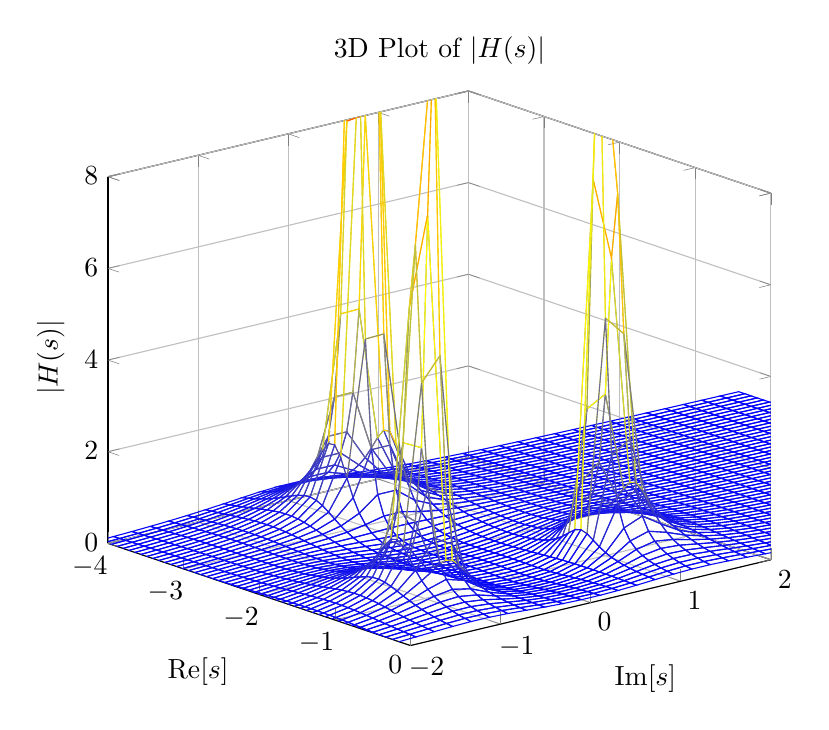
\begin{tikzpicture}
    \begin{axis}[
        view={50}{20},
        width=10cm,
        grid=major,
        xmin=-4, xmax=0,
        ymin=-2, ymax=2,
        zmin=0, zmax=8,
        xlabel={Re[$s$]},
        ylabel={Im[$s$]},
        zlabel={$|H(s)|$},
        title={3D Plot of $|H(s)|$},
        samples=50,
        domain=-4:0,
        y domain=-5:5
    ]
    \addplot3[mesh, shader=interp]
        {
            abs((x+1)*(x+1) + y*y) * abs((x+2)*(x+2) + y*y) / 
            (
                abs((x+3)*(x+3) + y*y) * 
                abs((x+1)*(x+1) + (y+1)*(y+1)) * 
                abs((x+1)*(x+1) + (y-1)*(y-1))
            )
        };
    \end{axis}
    \end{tikzpicture}
    
    \item Relationship between Transfer function and Frequency Response \\
    By substituting $s = j\omega$, we obtain
    \[\Tilde{H}(s)\Bigg|_{s=j\omega}=\Tilde{H}(j\omega)=\int^\infty_0h(t)e^{-j\omega t}dt\]
    By substituting $\omega = 2\pi f$, we obtain
    \[\Tilde{H}(j\omega)\Bigg|_{\omega=2\pi f} = \int^\infty_0h(t)e^{-j2\pi ft}dt\]
    Therefore, for a causal LTI system where $h(t) = 0$ when $t < 0$ , we have 
    \[H(f) = \Tilde{H}(j\omega)\Bigg|_{\omega = 2\pi f} = |\Tilde{H}(j\omega)|e^{j\angle \Tilde{H}(j\omega)}\]
    Thus we can conclude that
    \[x(t) = Ae^{j(\omega_0t+\psi)}\rightarrow\boxed{\Tilde{H}(j\omega)}\rightarrow y(t)=A|\Tilde{H}(j\omega_0)|e^{j(\omega_0t+\psi+\angle\Tilde{H}(j\omega_0))}\]
    \[x(t) = Acos(\omega_0t+\psi)\rightarrow\boxed{\Tilde{H}(j\omega)}\rightarrow y(t)=A|\Tilde{H}(j\omega_0)|cos(\omega_0t+\psi+\angle\Tilde{H}(j\omega_0))\]
    \[x(t) = Asin(\omega_0t+\psi)\rightarrow\boxed{\Tilde{H}(j\omega)}\rightarrow y(t)=A|\Tilde{H}(j\omega_0)|sin(\omega_0t+\psi+\angle\Tilde{H}(j\omega_0))\]
    \item System Stability \\
    Poles and Zeros : Poles are defined as the roots of the denominator polynomial of $\Tilde{H}(s)$, whenever $\Tilde{H}(\alpha) = \infty$, $\alpha$ is Pole of the system. Zeros are defined as the roots of the numerator polinomial of $\Tilde{H}(s)$, whenever $\Tilde{H}(\beta) = 0$, $\beta$ is Zero of the system.
    \begin{enumerate}
        \item BIBO Stable
        \begin{itemize}
            \item $\displaystyle\lim_{t \rightarrow \infty } h(t) = 0$
            \item All system poles lying on the left-half of s-plane.
        \end{itemize}
        \item Marginally Stable
        \begin{itemize}
            \item $\displaystyle \lim_{t \rightarrow \infty }|h(t)| \neq 0$ and $\displaystyle \lim_{t \rightarrow \infty}h(t) \neq 0$
            \item One or more system poles lying on the imaginary axis of the s-plan and no system pole lying on the right half s-plane. System poles lying on the imaginary axis must be distinct (non-repeated).
        \end{itemize}
        \item Unstable 
        \begin{itemize}
            \item $\displaystyle\lim_{t \rightarrow \infty } |h(t)| = \infty $
            \item One or more system poles lying on the right-half s-plane.
        \end{itemize}
    \end{enumerate}
\end{enumerate}
\subsubsection{First Order System}
\begin{enumerate}
    \item Differential Equation
    \begin{equation}
        T\frac{dy(t)}{dt}+y(t)=Kx(t)
    \end{equation}
    \[
        where = 
        \begin{cases}
            & x(t) : system\;input \\
            & y(t) : system\;output \\
            & K : DC\;Gain\\
            & T : time-constant
        \end{cases}
    \]
    \item Transfer Function \\
    By assuming zero initial conditions
    \begin{multline}
        TsY(s)+Y(s) = KX(s) \longrightarrow \Tilde{H}(s) = \frac{Y(s)}{X(s)}=\frac{K}{Ts+1} \\ 
    \end{multline}
    Poles: $s_1 = - \frac{1}{T}$
    \item Impulse Response $h(t)$
    \begin{equation}
        h(t) = \mathscr{L}^{-1}\{\Tilde{H}(s)\} = \frac{K}{T}e^{\frac{-t}{T}}u(t) 
    \end{equation}
    \begin{figure}[h]
        \centering
        \includegraphics[width=0.75\linewidth]{image/e2ba5c9507c51e791e37c061e3eef1a.png}
    \end{figure}
    \item Step Response $o(t)$
    \begin{align*}
        o(t) &=  \int^t_{-\infty}h(\tau)d\tau \\
         &= \mathscr{L}^{-1}\{\frac{1}{s}\Tilde{H}(s)\} \\
         &= K[1-e^{t\frac{t}{T}}]u(t)
    \end{align*}
    \begin{figure}[h]
        \centering
        \includegraphics[width=0.75\linewidth]{image/9e19b7ea507f2d6e90b842d6f5b0fac.png}
    \end{figure}
\end{enumerate}
\subsubsection{Second Order System}
\begin{enumerate}
    \item Differential Equation
    \begin{equation}
        \frac{d^2y(t)}{dt^2}+2\zeta\omega_n\frac{dy(t}{dt}+\omega_n^2y(t) = K\omega_n^2x(t)
    \end{equation}
    \[
    where = 
    \begin{cases}
        & x(t) : system\;input \\
        & y(t) : system\;output \\
        & \zeta : damping\;ratio\\
        & \omega_n : undamped\;natural\;frequency\;(when \zeta < 1) \\
        & K : DC\;Gain
    \end{cases}
    \]
    \item Transfer Function $\Tilde{H}(s)$
    \begin{multline}
        s^2Y(s)+s2\zeta\omega_nsY(s)+\omega_n^2Y(s) = K\omega_n^2X(s) \\
        \longrightarrow \Tilde{H}(s)=\frac{Y(s)}{X(s)} = \frac{K\omega_n^2}{s^2+2\zeta\omega_n s+\omega_n^2}
    \end{multline}
    Poles: $s_{1,2} = -\omega_n\zeta \pm \omega_n(1-\zeta^2)^{1/2}$ 
    \begin{itemize}
        \item $\zeta > 1 $ : $s_{1,2} = -\omega_n\zeta \pm \omega_n(1-\zeta^2)^{1/2}$ \\
        Poles are real and distinct. \\
        System is said to be \textbf{OVERDAMPED}
        \item $\zeta = 1$ : $s_{1,2} =-\omega_n$ \\
        Poles are real and repeated. \\
        System is sad to be \textbf{CRITICALLY DAMPED}
        \item $0<\zeta<1$: $s_{1,2} = -\omega_n\zeta \pm j\omega_n(1-\zeta^2)^{1/2}$ \\
        Poles are a complex conjugate pair. \\
        System is said to be \textbf{UNDERDAMPED}
        \item $\zeta = 0$ : $s_{1,2} =-j\omega_n$ \\
        Poles are pure-imaginary conjugate pair. \\
        System is said to be \textbf{UNDAMPED}
    \end{itemize}
    \item Impulse Response and Step Response
    \begin{enumerate}
        \item Overdamped System ($\zeta > 1$)
    \end{enumerate}
\end{enumerate}